% THIS IS A LATEX TEMPLATE FILE FOR PAPERS INCLUDED IN THE
% *Anthology of Computers and the Humanities*. ADD THE OPTION
% 'final' WHEN CREATING THE FINAL VERSION OF THE PAPER. 
% DO NOT change the documentclass
%\documentclass[final]{anthology-ch} % for the final version
\documentclass{anthology-ch}         % for the submission

% LOAD LaTeX PACKAGES
\usepackage{booktabs}
\usepackage{graphicx}
\usepackage{amsmath}
\usepackage{float}
\usepackage{adjustbox}
\usepackage{fancyvrb}
\usepackage{svg}
\usepackage{comment}
\usepackage[inkscapelatex=false]{svg}
% ADD your own packages using \usepackage{}
\usepackage{cleveref}
\usepackage{paralist}


\newcommand{\joseph}[1]{\textcolor{blue}{Joseph:~#1}}
\newcommand{\marie}[1]{\textcolor{red}{Marie:~#1}}
\newcommand{\joel}[1]{\textcolor{purple}{Jo{\"e}l:~#1}}


% TITLE OF THE SUBMISSION
% Change this to the name of your submission
\title{Producing Structured Data from Historical Sources:\\a Preliminary Application to French Senate \textit{Tables}}
%% ou aussi "…: Experiments on French Senate Tables"
%% ou: "From Historical Sources to Structured Data: …"

% AUTHOR AND AFFILIATION INFORMATION
% For each author, include a new call to the \author command, with
% the numbers in brackets indicating the associated affiliations 
% (next section) and ORCID-ID for each author.  
\author[1,2]{Jo{\"e}l F{\'e}eral}[
  orcid=0009-0005-6646-0733
]

\author[1]{Joseph Chazalon}[
  orcid=0000-0002-3757-074X
]

% While we encourage including ORCID-IDs for all authors, you can
% include authors that do not have one by definining an empty ID.
\author[1]{Marie Puren}[
  orcid=0000-0001-5452-3913
]

% There should be one call to \affiliation for each affiliation of
% the authors. Multiple affiliations can be given to each author
% and an affiliation can be given to multiple authors. 
\affiliation{1}{EPITA Research Lab, Le Kremlin-Bic{\^e}tre, France}
\affiliation{2}{{\'E}cole des Chartes, Paris, France}

% KEYWORDS
% Provide one or more keywords or key phrases seperated by commas
% using the following command
\keywords{Parliamentary Archives, Structured Data, Generative Models, Evaluation}

% METADATA FOR THE PUBLICATION
% This will be filled in when the document is published; the values can
% be kept as their defaults when the file is submitted
\pubyear{2025}
\pubvolume{1}
\pagestart{1}
\pageend{1}
\conferencename{Proceedings of Conference XXX}
\conferenceeditors{Editor1 Editor2}
\doi{00000/00000}  

\addbibresource{bibliography.bib}

%%%%%%%%%%%%%%%%%%%%%%%%%%%%%%%%%%%%%%%%%%%%%%%%%%%%%%%%%%%%%%%%%%%%%%%%%%%
% HERE IS THE START OF THE TEXT
\begin{document}

\maketitle

\begin{abstract}
We address the extraction of structured data from noisy historical documents (namely, the 1931 \textit{Tables nominatives} of the French Senate) using a LLM guided by lightly constrained generation rather than strict post‑hoc validation. Our contribution is threefold: (1) a minimal, application‑driven target schema (speaker name + list of page references) expressed so it can be injected into the prompt to steer generation; (2) a hybrid pipeline that decouples OCR from schema‑oriented generation, leveraging the LLM’s tolerance to OCR noise while limiting hallucinations via an expected JSON format; (3) an evaluation protocol for structured outputs using optimal record matching and a continuous Integrated Matching Quality metric that overcomes precision/recall brittleness.

%A real case study on early 20th‑century parliamentary index pages illustrates how prompt and schema choices act as critical meta‑parameters in performance. This approach supports scalable, transparent construction of structured historical corpora.

Code and data will be released publicly. During the review phase, they are available at \url{https://anonymous.4open.science/r/Evaluate-Structured-Output-F295}.
\end{abstract}

%\section*{Acknowledgements}
%\textit{Omitted during review phase.}
% TODO thank BnF / Mezanno project funding

\section{Introduction}
\label{sec:intro}
The growing use of artificial intelligence by historians \cite{clavert2024histoire} is multiplying the possibilities for producing historical datasets. The advent of large language models (LLMs) is further changing the landscape, especially for processing textual data corpora, with a proliferation of uses and experiments in the humanities and social sciences\footnote{The "DH@LLM: Grands modèles de langage et humanités numériques" conference program, held in Paris in July 2025, is a good illustration of this: \href{https://www.crihn.org/nouvelles/2025/01/16/colloque-dhllm-grands-modeles-de-langage-et-humanites-numeriques-sorbonne-universite/}{https://www.crihn.org/nouvelles/2025/01/16/colloque-dhllm-grands-modeles-de-langage-et-humanites-numeriques-sorbonne-universite/}}. Zero-shot LLMs are capable of performing a wide range of tasks without the need for task-specific examples or fine-tuning \cite{kojima2022large,wei2022emergent,zhao2023survey} and have demonstrated their ability to carry out many time-consuming tasks in historical research, such as transcription \cite{humphries2024unlocking}, information extraction \cite{knutsen2024alimenter}, or annotation \cite{yuan2025leveraging}. 

%In the context of historical data extraction, a key issue is obtaining structured outputs. While structured generation -- which constrains a Large Language Model to directly produce information in a predefined format like JSON -- is a way to achieve this, a structured output can also be obtained through post-processing of free-form text generation. Regardless of the method, structured output enables the preservation of \joseph{the link to?} the original document and facilitates return to the source, while still allowing for subsequent processing — such as, for instance, integration into a database.

The use of large language models (LLMs) opens new perspectives for extracting structured data \cite{liu2024structured} from historical documents. In the context of historical data extraction, a central challenge lies in obtaining structured outputs. One approach is structured generation, which constrains a large language model to directly produce information in a predefined format such as JSON. Alternatively, structure can be imposed through post-processing of free-form text outputs. Regardless of the approach, producing structured data enables traceability back to the original document and facilitates source verification. It also supports downstream uses, such as integration into a database or further computational analysis.

%\joseph{Est-ce que le problème n'est pas de dire : 1. comment on passe du texte brute au CSV (pour simplifier) et 2. comment on évalue ce que ça donne ?}

%\marie{Si ça vous convient à tous les deux, je trouve ça mieux.}
%\joel{Oui, ça me convient !} \marie{Ci-dessous, une proposition, en ayant utilisé ce qu'a dit Joseph. J'ai aussi utilisé ce qu'il a dit par Teams.}

Two fundamental issues still remain: (1) how to move from raw text to an exploitable structured representation, such as a table or CSV file ; and (2) how to assess the quality and reliability of the extracted data. This article addresses both aspects through a concrete case study: the extraction of structured information from the 1931 \textit{Tables nominatives} or \textit{Tables des noms} of the French Senate (index of senatorial activity ordered by name). We explore a lightly constrained generation approach using an LLM and propose a method to represent the target data, guide the extraction process, and evaluate system performance. Beyond this specific case, the study aims to contribute to broader reflections on the feasibility and limitations of generative models for structuring historical data.

The \textit{Tables des noms} of the French Senate was published during the French Third Republic (1870–1940)\footnote{These tables are part of the \textit{Tables annuelles} (yearly activity index), which can be consulted on the digital library of the French national library (\textit{BnF}): \href{https://gallica.bnf.fr/ark:/12148/cb371291967/date.item}{https://gallica.bnf.fr/ark:/12148/cb371291967/date.item}.}.
Within the broader documentary ecosystem of the \textit{Journal Officiel} ---~which seeks to reconstruct parliamentary activity and its legal or regulatory outcomes in France~---, the Senate's \textit{Tables nominatives} offer a concise and systematic record of senators' interventions during public sessions.
These indexes were designed to accompany the transcription of debates\footnote{The complete transcriptions of Senate debates can be consulted via Gallica: \href{https://gallica.bnf.fr/ark:/12148/cb34363182v/date}{https://gallica.bnf.fr/ark:/12148/cb34363182v/date}.} and to facilitate their consultation.
Manually compiled once a year, they recorded each intervention by senators or members of the government who spoke during the sessions, the subject of their speech, and the corresponding page number.
%
While these tables were particularly useful at a time when full-text search in digitized parliamentary debates was not possible, they still hold significant value for historians today.
Systematically extracting data from them would make it possible to track parliamentary activity over the long term, quantify the interventions of specific senators affiliated with particular political movements, or support the cross-validation of named entities extracted from the debates themselves.
%
Our objective is to extract structured data from these \textit{Tables}; for our initial experiments, we focus on a single \textit{Table nominative}, namely that of 1931.
The early 1930s marked the beginning of the decline of French parliamentarism, culminating in the fall of the Third Republic in 1940 \cite{morel2024parlement}. Analyzing the 1931 \textit{Table} allows us to lay the groundwork for a broader study that will extend across the entire decade, with the aim of capturing the parliamentary activity of the Senate and, subsequently, of the Chamber of Deputies.


%\textbf{Problem:} \textit{[bon là, la 1ère phrase, j'ai un peu riffé... Je ne sais pas si c'est vrai]} Yet, the evaluation of these outputs remains dominated by symbolic “exact match” metrics: Exact Match, Precision/Recall/F-score at the node or parent-child pair level. These metrics are blind to semantic proximity: a predicted label that differs by just one level in the hierarchy or by a lexical variant is penalized as heavily as a completely unrelated prediction, which distorts the measurement of actual performance.

%\joseph{Partie trop technique pour l'intro selon moi, à déplacer dans la partie "Evaluation Framework"}

%\marie{Dans ce cas, il faut supprimer la Research question et enchaîner direct ensuite sur Case study}

%\textbf{Hypothesis:} Optimal Transport (OT) provides a mathematical framework to measure the minimal cost of transforming one distribution into another: here, the distribution of labels generated by the LLM versus the ground truth. By assigning a cost proportional to the semantic/hierarchical distance between labels, OT softens the penalty: the closer the prediction, the lower the cost. The originality of this case study lies in the combination of OT + structured output, which is rarely explored for document indexing tasks. 

%\textbf{Research question:} To what extent does Optimal Transport offer a more fine-grained, human-aligned evaluation than classical metrics when assessing the structured output of an LLM on a document indexing task?

%\textbf{Case study:} Senate tables. Brief presentation of the source and its usefulness.


After reviewing existing approaches to structured data extraction and evaluation (Section~\ref{sec:related-work}), we present three main contributions.

\section{Related Work}
\label{sec:related-work}

Building upon our initial argument, we structure our review around three key questions: 
\begin{inparaenum}[(1)]
    \item How can structured data be effectively modeled? 
    \item How can the quality of structured data produced by such approaches be evaluated? 
    \item How can structured data be generated from text?
\end{inparaenum}

\subsection{Modeling Structured Data}
\label{sec:modeling-structured-data}

Structured data can take various forms, including: 

\textbf{Record Sets:} These are unordered sets of tuples, similar to database tables where columns represent attributes of objects. This structure is commonly employed in Information Extraction tasks, such as named entity recognition~\cite{nadeau_survey_2007} or relation extraction~\cite{mintz_distant_2009}.

\textbf{Record Sequences:} These are ordered versions of record sets, where the sequence of records holds significance. The order may reflect criteria such as time or facilitate tasks like cross-validation, as seen in directories.

\textbf{Trees:} These hierarchical structures are often used to represent nested relationships or dependencies, such as in dependency parsing~\cite{de-marneffe-etal-2014-universal}.

\textbf{Graphs:} These are flexible structures used to represent consolidated knowledge, such as ontologies or knowledge graphs. While these are widely studied, their evaluation typically falls outside the scope of Information Extraction and is beyond the focus of this work.

In this paper, we focus on record sets and sequences, as they are the most relevant for our case study involving the extraction of structured data from parliamentary documents. The various models we experimented with are described in~\Cref{sec:documents-approach}.

\subsection{Evaluating the Quality of Structured Data}
\label{sec:evaluating-structured-data}

The evaluation of structured data quality can be broadly categorized into two types of metrics: edit distance metrics and matching metrics, as defined in~\cite{chen_unified_2023}.

\textbf{Edit Distance Metrics:}  
These metrics involve complex optimization processes and are often computationally intensive. Additionally, their interpretability is limited, as they do not provide a direct comparison between the produced and expected data. Examples include the classical Levenshtein distance for character-level comparisons and Tree-Edit Distance~\cite{zhang_simple_1989} for tree structures. While general graph edit distance metrics exist, their complexity often renders them impractical for real-world applications.

\textbf{Matching Metrics:}  
Matching metrics are more interpretable, as they explicitly identify the elements that match between the produced and expected data. Most approaches rely on bipartite matching between the predicted and reference data sets, computing scores based on the number of matched elements~\cite{chen_unified_2023}. Common metrics include the F1 score, which combines precision and recall, and the Jaccard index, which measures set similarity. However, fewer studies address structured data or partial matching, where the produced data may not perfectly align with the expected data. 
It is interesting to note that the computer vision community share the exact same problem, and a similar framework is proposed in the context of the COCO Panoptic Segmentation Challenge~\cite{kirillov_panoptic_2019}. The evaluation protocol relies on an optimal matching between the surfaces of the predicted and ground truth segmentations to jointly evaluate detection, segmentation and classification of regions ---~which is similar to the approch of Chen et al.~\cite{chen_unified_2023}.

In our work, we adopt a matching metric based on optimal matching between structured data sets, which generalizes the bipartite matching approach while accommodating partial matches. This approach not only provides a quantitative evaluation of data quality but also identifies missed or hallucinated elements, offering actionable insights.

\subsection{Producing Structured Data from Text}
\label{sec:producing-structured-data}

Approaches for generating structured data from text can be broadly divided into two categories: detection-based (extractive) and generation-based (generative or abstractive).

\textbf{Detection-Based Approaches:}  
These methods focus on identifying text fragments corresponding to specific fields or elements of the structured data. Traditional approaches relied on rule-based methods, such as regular expressions or heuristics. More recently, machine learning models, such as sequence labeling models (e.g., CRF-based methods~\cite{finkel_incorporating_2005}) or transformer-based encoder-only models (e.g., BERT~\cite{devlin-etal-2019-bert}), have become prevalent. Transformer-based models are particularly effective due to their intrinsic capabilities and their ability to be fine-tuned on specific tasks with relatively small datasets. Additionally, their design enforces strict alignment between input text and output labels, reducing the risk of hallucinations (i.e., generating data not present in the input). However, these approaches require task-specific training, which demands data, computational resources, expertise, and time.

\textbf{Generation-Based Approaches:}  
These methods leverage autoregressive models to generate structured data by ``translating'' the input text into the desired format. The advent of LLMs has spurred interest in this approach due to their impressive generalization capabilities across diverse tasks without requiring task-specific training~\cite{radford_improving_2018,radford_language_2019,brown_language_2020}. Outputs can be constrained to specific formats, such as JSON, or more complex structures, as long as the set of valid tokens can be dynamically computed~\cite{willard2023efficient}. These models can produce complex, nested structures by generating elements sequentially and can infer implicit elements not explicitly present in the input text. However, their primary drawback is their susceptibility to hallucinations, which are challenging to detect.

In this paper, we explore the effectiveness of generation-based approaches for handling repetitive structures in parliamentary indexes or \textit{Tables}. We leverage the zero-shot capabilities of LLMs and evaluate the viability of this approach for generating structured data in this specific context.

% Note: Hybrid approaches, which combine detection-based and generation-based methods (e.g., using LLMs to generate training data for detection-based models), exist but require significant computational resources and expertise. These approaches are beyond the scope of this work.

\section{Schema-Guided Extraction of Parliamentary Interventions from Historical Indexes}
\label{sec:documents-approach}

\subsection{The 1931 \textit{Tables nominatives} of the French Senate}
There is an edition of the \textit{Tables du Journal Officiel} for each year, typically comprising around 450 pages in the 1930s. The section entitled \textit{Tables des noms}—which includes both the Senate and the Chamber of Deputies—spans approximately forty pages, with the Senate portion generally covering around fifteen. For the year 1931, the Senate's \textit{Tables des noms} consists of 14 pages and roughly 300 entries, each corresponding to an intervention in the assembly.
Each entry is associated with a speaker and details various types of actions (requests for interpellation, bill discussions, reading of committee reports, submission of amendments, etc.), along with a page reference directing the reader to the full transcription of the intervention. These transcriptions are published in the Senate's \textit{Débats parlementaires}. The \textit{Tables} are therefore functionally linked to the transcriptions through page numbers. Moreover, as pagination is continuous throughout the year, each page reference makes it possible to accurately determine the date of the corresponding intervention.


%\joseph{insérer une image pour illustrer ? voir le faire dès l'introduction !}


\subsection{Pipeline for Schema-Guided Structured Data Extraction}

Despite recent advances in Large Vision-Language Models (LVLMs), their end-to-end, zero-shot performance remains insufficient for high-accuracy OCR tasks. To address this, we adopt a straightforward pipeline that leverages the strengths of specialized components to maximize overall extraction accuracy.

First, each page image is processed independently using the PERO OCR engine~\cite{kodym2021layout,kis2021atst,kohut2021tsnet} to detect and transcribe text. Given the persistent challenges in general page layout segmentation, we generate three transcription variants per page to capture the variability inherent in such pipelines. Such variants will be described in more detail in \Cref{sec:xp-dataset}.

Once the text for each page is obtained, we concatenate the transcriptions from all relevant pages to form a single text stream. This aggregated text is then provided as input to a Large Language Model (LLM), which is instructed to produce the target structured data. For practical reasons, we process each page independently, but the approach is readily extensible to multi-page contexts.

\begin{figure}[tb!]
  \centering
   %
\includegraphics[width=\textwidth]{img/simple_pipeline.png}
  %\includesvg[width=\textwidth]{img/simple_pipeline.svg}
   
\includegraphics[width=0.95\textwidth]{img/pipeline.pdf}
  \caption{Document processing pipeline. The input to the LLM consists of the concatenated OCR-extracted raw text, a natural language prompt, and a predefined schema describing the target structure. The LLM generates a structured JSON object as output.
  %\joseph{Replace with the vector version of the figure (PDF). Clearly indicate that the LLM input consists of the concatenated page text, the prompt, and the schema, and that the output is a JSON object. Second gray box should be named "LLM".}
  }
  \label{fig:schema_pipeline}
\end{figure}

While LLMs can be prompted to generate structured outputs, it is essential to constrain their generations to match the expected format. Several methods exist for enforcing such constraints; the most effective to date involves filtering valid tokens during inference using an external validator, such as a finite state automaton~\cite{willard2023efficient}. This capability is available in the extended APIs of several commercial models.

Our information extraction process thus relies on submitting OCR-processed text to the LLM and obtaining output that conforms to a predefined JSON schema. This setup requires three key components: \textbf{a data schema}, \textbf{a prompt}, and \textbf{an API supporting constrained output}.

For this study, we selected the Mistral API\footnote{The Mistral API Documentation is available at \url{https://docs.mistral.ai/api/}.}, using the Ministral 8B Instruct v2410 model~\cite{MistralAI2024Ministral8B}. This choice is motivated by the model's strong zero-shot performance, cost-effectiveness, and the public availability of its weights for research purposes\footnote{Ministral 8B weights are available at \url{https://huggingface.co/mistralai/Ministral-8B-Instruct-2410}.}.


\subsection{Data Modeling and Schema Definition}
\label{sec:approach-datamodel}

The primary goal of this study is to extract structured information on parliamentary activity in the French Senate for the year 1931, with the practical objective of building an interactive timeline that visualizes the density of interventions over time. To ensure the reliability and interpretability of this timeline, it is crucial to provide clear indicators of extraction quality.

Directly linking extraction reliability to the confidence in answering historical research questions remains an open challenge. Therefore, we focus our evaluation on well-defined metrics that quantify the similarity between the predicted intermediate data structure and a reference (ground truth) structure. While these metrics do not yet account for the semantic impact of each error, they offer a transparent basis for assessing extraction performance.

The core extraction task centers on identifying individual entries in the \textit{Tables nominatives} ---~specifically, the names of senators and their associated page references. These page numbers serve as indirect temporal markers, as the source documents use continuous pagination throughout the year. The extracted information is represented in JSON format, which is both structured and interoperable, facilitating downstream processing and conversion to tabular formats (e.g., CSV). Figure~\ref{fig:json_struct} illustrates the target output structure.

\begin{figure}[tb!]
\centering
\small
\begin{verbatim}
{
  "list_of_speakers": [
    {
      "name": "Dentu",
      "page_references": [
        1024,
        1031,
        1560,
        1563,
        1564
      ]
    },
    {
      "name": "Desjardins (Charles)",
      "page_references": [
        563
      ]
    }
  ]
}
\end{verbatim}
\caption{Example JSON output representing structured data extracted from the \textit{Tables nominatives}. Each entry corresponds to a participant (e.g., a senator) and a list of page numbers where they are mentioned. These references act as temporal markers due to the continuous pagination of the source. For simplicity, intervention categories are omitted in this study. %\joseph{Consider moving this figure to the introduction for a general overview.}
}
\label{fig:json_struct}
\end{figure}

The data schema guiding LLM inference is defined at the granularity of speaker names and their corresponding page references, which suffices for constructing the intended timeline. We use Pydantic\footnote{Pydantic documentation is available at \url{https://docs.pydantic.dev}.}, a Python library for data modeling, to specify the schema in a JSON-compatible format with strict type validation and embedded descriptions. These description fields serve as semantic tags, enhancing both prompt clarity and LLM guidance. Figure~\ref{fig:pydantic_schema} (see \Cref{appdx:schema}) presents the simplified schema used in this work.

%     page_references: Union[List[int], str] = Field(..., 
% ↑ general model which can handle cross-references

\subsection{Prompting the LLM for Structured Data Extraction}

The prompt provided to the LLM (see \Cref{appdx:full-prompt}) is designed to guide the extraction of political participants—primarily senators and ministers—and their associated page references from the input text. Its structure is as follows:

\begin{itemize}
  \item \textbf{Task Definition:} The prompt clearly states that the input consists of entries, each corresponding to an individual involved in Senate activities (e.g., senators, ministers), and that the goal is to extract their names and the page numbers referencing their interventions.
  \item \textbf{Key Term Clarification:} Definitions are provided for essential terms such as ``entries'' and ``actions'' to ensure unambiguous interpretation.
  \item \textbf{Handling Special Cases:} The prompt specifies procedures for cases such as index cross-references (where no page numbers are given, only a reference to another entry) and split entries spanning multiple pages (which are to be ignored in this preliminary study to maintain extraction simplicity).
  \item \textbf{Formatting Instructions:} Explicit guidelines are given for representing names (e.g., first names in brackets after last names) and formatting page references.
\end{itemize}

Optionally, the prompt could be further improved by incorporating additional historical context or representative examples (few-shot prompting).


\subsection{Iterative Refinement of the Data Model and Prompt}
Both the data schema and the extraction prompt underwent iterative refinement during this study. This process was motivated by the observation that the LLM occasionally proposed alternative, and sometimes more effective, ways of structuring the extracted information than initially anticipated. For instance, the model would naturally deduplicate repeated page references for a given speaker, streamlining the output beyond the original schema specification. Consequently, the construction of the ground truth required a balance between adhering to formal schema constraints and accommodating the LLM’s practical structuring tendencies.

To ensure unbiased evaluation, all schema and prompt adjustments were based exclusively on performance observed on a single development page (referred to as \textbf{``page 02''} in experiments), with the remaining pages reserved for final testing. This approach aligns with standard machine learning practice, maintaining a clear separation between development and evaluation data.

Future work could automate this refinement loop or incorporate more systematic prompt engineering strategies.

\section{Experiments}
\label{sec:experiments}
The evaluation setup was established through an initial development phase, during which the data model, prompt instructions, and reference structured data for a selected development page were iteratively refined. After finalizing this phase, we applied the baseline model to a broader set of pages and manually corrected the outputs to construct an unbiased ground truth for evaluation.

This section details the resulting dataset, the variants generated for analysis, and the evaluation protocol employed to rigorously assess prediction quality.


\subsection{Dataset}
\label{sec:xp-dataset}

% Overview of dataset construction
Ground truth data were constructed to rigorously evaluate extraction quality across varying levels of OCR text fidelity. For each selected page, three distinct OCR variants were generated using the PERO OCR engine~\cite{kis2021atst,kodym2021layout,kohut2021tsnet}:
\begin{inparaenum}[(1)] 
    \item a manually corrected version serving as the gold standard, 
    \item a version with manual layout segmentation, and 
    \item a raw, uncorrected OCR output.
\end{inparaenum}
This design enables systematic assessment of the extraction pipeline’s robustness to noise and layout artifacts.

% Page sampling and annotation protocol
A random sample of five sequential pages was selected for manual transcription and annotation. Because pages are not necessarily contiguous, some speaker entries may be incomplete; in such cases, the LLM was instructed to omit these partial elements. This setup reflects realistic extraction challenges, as entries may span multiple pages. (Handling such cases in production would require multi-page or streaming input, which is beyond the scope of this study.)

% Extraction and evaluation protocol
Each page was processed independently to avoid optimistic bias from sequential context. This sometimes resulted in extractions starting mid-entry, providing the LLM with truncated information and highlighting its ability to interpret partial context. Although the source documents are generally well-digitized, occasional distortions (e.g., page folds) and fragmented input introduce realistic difficulties, exposing model limitations in non-ideal conditions.

% Output generation and schema constraints
Structured outputs were generated using the Ministral 8B model, with a fixed prompt and a Pydantic schema to enforce output consistency. A temperature of zero was used to ensure deterministic results. For each page and OCR variant, the model produced structured JSON outputs, which were then compared to manually curated ground truth representations.

% Summary statistics
The evaluation covers 109 entries across five pages, with each entry assessed for all three OCR conditions.




\subsection{Structured Output Evaluation Protocol}
The evaluation aims to rigorously assess the structured outputs generated by the LLM (denoted as $P$) against a manually curated ground truth ($G$). As described in \Cref{sec:approach-datamodel}, each data instance consists of a \textbf{list of speaker entries}, where each entry comprises a \textbf{speaker name} and a \textbf{list of pages} referencing their speeches.

A key challenge arises from the fact that the model may produce the correct set of entries but in a different order, or with minor structural variations. To address this, we adopt a flexible alignment strategy inspired by prior work~\cite{chen_unified_2023,kirillov_panoptic_2019}, leveraging optimal transport to establish a one-to-one correspondence between predicted and ground truth entries. This approach accommodates order invariance and tolerates minor discrepancies, enabling a robust evaluation of extraction quality.

\subsubsection{Entry-level Distance and Optimal Assignment}
To rigorously compare predicted and ground truth entries, we define a normalized entry-level distance function that quantifies the similarity between each pair.

For the textual component (senator name), we compute the Ratcliff/Obershelp distance, which measures the similarity based on the longest common subsequence, after lowercasing and trimming whitespace. This yields a normalized distance $d_n(g_i, p_j) \in [0, 1]$, where 0 indicates an exact match and 1 indicates complete dissimilarity.

For the list of referenced pages, we use the Intersection-over-Union (IoU) set distance:
$$
d_p(g_i, p_j) = 1 - \frac{|\text{ref\_pages}(g_i) \cap \text{ref\_pages}(p_j)|}{|\text{ref\_pages}(g_i) \cup \text{ref\_pages}(p_j)|}.
$$

The overall entry distance is defined as the product of these two components:
$$
d_e(g_i, p_j) = d_n(g_i, p_j) \times d_p(g_i, p_j).
$$

To establish a one-to-one correspondence between predicted and ground truth entries, we employ optimal transport~\cite{peyré2020computationaloptimaltransport}. This approach finds the assignment that minimizes the total distance across all pairs, accommodating order invariance and structural discrepancies. The resulting alignment provides a principled basis for evaluating extraction quality at the entry level.


\subsubsection{Limitations of Standard Metrics: Precision, Recall, and F1-Score}

Conventional metrics such as \textbf{precision}, \textbf{recall}, and \textbf{F1-score} are widely used to evaluate extraction tasks. Precision quantifies the proportion of correctly generated entries among all model outputs, while recall measures the fraction of ground truth entries successfully retrieved. The F1-score, as their harmonic mean, is intended to provide a balanced summary of performance.

However, in our evaluation protocol—where predicted and ground truth entries are aligned one-to-one using optimal transport—these metrics become unreliable. The injective nature of the alignment ensures that the number of predicted entries always matches the number of ground truth entries. As a result, precision is trivially maximized, regardless of the actual quality of the matches, and recall fails to reflect missing or spurious entries, since all elements are forcibly paired. Consequently, the F1-score inherits these distortions, leading to an inflated and potentially misleading assessment of model performance.

\subsubsection{Integrated Matching Quality (IMQ): A Robust Evaluation Metric}

While standard metrics fail to capture the nuanced quality of structured matches, our protocol leverages the entry-level distance $d_e$ to quantify the fidelity of each aligned pair. For each match, we define a quality score $q_i = 1 - d_e(g_i, p_i)$, where $q_i \in [0, 1]$ reflects the closeness of the predicted entry to its ground truth counterpart.

Rather than imposing an arbitrary threshold to classify matches as correct or incorrect, we adopt an area-under-curve (AUC) approach to aggregate match quality across all possible thresholds. Specifically, for each threshold $t \in [0, 1]$, we compute the proportion of matches with $q_i \geq t$:
$$
F(t) = \frac{1}{n} \sum_{k=1}^{n} \mathbb{1}_{q_k \geq t}
$$
The \textbf{Integrated Matching Quality (IMQ)} is then defined as the area under this curve:
$$
\text{IMQ} = \int_{0}^{1} F(t) \, dt
$$

IMQ provides a comprehensive summary of extraction quality, rewarding both the number and the closeness of matches. A score of 1 indicates perfect alignment, while lower values reflect increasing divergence. This continuous, threshold-free metric is particularly well-suited to evaluating LLM outputs, where minor deviations are common even under strong structural constraints. IMQ thus enables a principled, fine-grained assessment of structured extraction performance.

%%%%%%%%%%%%%%%%%%%%%%% !!! %%%%%%%%%%%%%%%%%%%%
\begin{comment}
\subsection{Qualitative Analysis via Matching Scores}
\joseph{only include / rephrase these ideas if we manage to include some qualitative analysis in \Cref{sec:results}!}
The entry-level matching scores produced by our evaluation protocol provide direct insight into extraction errors. Low-quality matches—those with low similarity scores—highlight cases where the model either hallucinated content or failed to extract a ground truth entry. By inspecting these specific alignments, we can efficiently diagnose systematic errors or challenging cases in the extraction process.
\end{comment}

\section{Results and Analysis}
\label{sec:results}
%\joseph{les tables de résultats doivent être générées automatiquement pour éviter les erreurs de copier-coller. Il faut exporter les données au format pandas, et utiliser Dataframe.to\_latex(). Je suggère de diviser en 3 tableaux pour plus de simplicité, et d'en mettre en annexe si nécessaire (après tout la version avec OCR "réaliste" est la plus représentative de ce qu'on peut espérer en production, non ?)}

We applied our matching method to five different pages (109 entries), each processed independently and exhibiting varying OCR qualities. The table below presents the results for each OCR-scanned page ---~processed without segmentation or correction~--- along with the corresponding sizes of the ground truth and predicted sets, and the number of matches ultimately selected by optimal transport.

\begin{adjustbox}{width=\textwidth, center}
\begin{tabular}{lrrrrrr}
\toprule
Source & Precision (Biased) & Recall (Biased) & IMQ & Ground Truth Entries & Predicted Entries & Matches \\
\midrule
page 02 & 1.0000 & 0.9565 & 0.9059 & 23 & 22 & 22 \\
page 03 & 1.0000 & 1.0000 & 0.8928 & 25 & 25 & 25 \\
page 04 & 1.0000 & 1.0000 & 0.9591 & 19 & 19 & 19 \\
page 05 & 1.0000 & 1.0000 & 0.8636 & 19 & 19 & 19 \\
page 10 & 1.0000 & 1.0000 & 0.8193 & 23 & 23 & 23 \\
\bottomrule
\end{tabular}

\end{adjustbox}
\newline

All pages exhibit perfect biased precision and recall; however, as previously discussed, these metrics are inherently limited in our context. Since they are directly derived from the optimal assignment ---~enforcing a one-to-one matching between the two sets, at least when they are of equal size~--- they do not fully reflect alignment quality.

The IMQ, on the other hand, offers a more nuanced assessment by capturing the distribution of match quality across all possible thresholds. For all processed pages, IMQ scores remain consistently high (ranging from 0.8193 to 0.9591), reflecting a strong homogeneity among correspondences. The IMQ also indirectly assesses the quality of the predicted dataset: not only are the matches structurally complete, but they also maintain an overall high level of semantic and syntactic proximity. Thus, the IMQ can be interpreted as a hybrid metric, functioning as a qualitative recall indicator while also integrating a proxy for precision, through penalization of low-quality matches.

Minor variations are observed across pages. Pages 5 and 10 show somewhat lower IMQ scores, likely due to document-specific typographic inconsistencies. On these pages, a significant number of first names are not enclosed in parentheses following the last names, contrary to the formatting assumed in the ground truth. Specifically, 21\% of entries on page 5 and 39\% on page 10 exhibit this discrepancy, compared to 0\% on the other pages. This typographic variation increases the string comparison cost and negatively impacts match quality.

Page 3, although exhibiting perfect biased recall and precision, has a slightly lower IMQ (0.8928). This may be attributed to OCR quality issues, particularly a fold in the gutter that introduces visual noise and degrades recognition performance.

Conversely, page 2 shows a high IMQ (0.9059), despite an imperfect recall. This is likely due to a sampling bias, as the prompting process for the LLM was initially designed with the structure of this specific page in mind. Accordingly, the strong performance on this page should be interpreted cautiously, as it does not necessarily generalize to the others. However, we can see that the device adapts well to page 4, which has the best score.

The 95.65\% recall on page 2 stems from a specific edge case in the source document, where an individual is listed twice (once as a senator and once as a minister). This leads to two distinct entries in the ground truth, while the LLM output consolidates them into a single prediction. We chose to preserve this functional distinction in the ground truth, while the model opted to factorize the information. This weakness is therefore linked to the design of the ground truth.

For comparison with the deemed-perfect OCR:

\begin{adjustbox}{width=\textwidth, center}
\begin{tabular}{lrrrrrr}
\toprule
Source & Precision (Biased) & Recall (Biased) & IMQ & Ground Truth Entries & Predicted Entries & Matches \\
\midrule
page 02 & 1.0000 & 1.0000 & 0.9513 & 23 & 23 & 23 \\
page 03 & 1.0000 & 1.0000 & 0.9430 & 25 & 25 & 25 \\
page 04 & 1.0000 & 1.0000 & 0.9821 & 19 & 19 & 19 \\
page 05 & 1.0000 & 1.0000 & 0.8778 & 19 & 19 & 19 \\
page 10 & 1.0000 & 1.0000 & 0.8966 & 23 & 23 & 23 \\
\bottomrule
\end{tabular}
\end{adjustbox}

Performance is better overall. The potentially superior performance of the noisy OCR might stem from its capture of running headers at the top of pages, providing better context in situations where entries at the beginning of a page are truncated. In the case of page 2, the LLM reproduced the repetition and thus the distinction between a senator holding two functions. This drop in results is less linked to the LLM's superior performance in a noisy context than to a better alignment of its behavior with the ground truth's expectations.

Consequently, there would also be a need to evaluate the prompt subsequently, as it is a crucial parameter for avoiding these errors. It's worth noting, however, that bypassing these exceptions in a massive extraction scenario would imply perfect knowledge of specific cases, which can be typographical or related to highly situational institutional choices. A schema with a reasonable degree of granularity and generic prompting allows for obtaining results that can be reasonably trusted, without requiring atomic knowledge of the documents' form. The calculation of statistics per page also offers bundles of clues about internal exceptions within the document structure, which can be significant.
%\begin{itemize}
 %   \item Comparative metric table (?)
  %  \item Analysis of metric relevance
%\end{itemize}
\section{Conclusion}
This work explored using large language models for structured data generation from historical sources, focusing on a specific case study, namely the 1931 \textit{Tables nominatives} of the French Senate. The approach ---~combining OCR, schema-guided structuring, and constrained generation via LLM~--- produced results evaluated with a more appropriate metric for an optimal alignment protocol, linking reference data with predicted data. The introduction of the IMQ metric was particularly crucial, allowing us to assess structuring quality beyond the traditional precision/recall scores, which are inadequate in this context.

Several avenues emerge for strengthening the approach's robustness and generalization. A central challenge, already noticeable in this work, lies in better connecting response hypotheses to research questions with automatically produced intermediate data. This will allow for evaluating their long-term robustness concerning the production process. Conversely, evaluating the prompt itself remains to be done to achieve a truly complete evaluation protocol. In any case, data structuring cannot be considered a simple, neutral pre-processing step: it dictates the form of possible historical analyses.

From this perspective, the prompt and the data model must be considered as ``meta-parameters'' of the entire historical data production system. It becomes essential to conceptualize their generation and adjustment as an integral part of the historical data processing chain. A promising path would involve systematizing and automating this meta-optimization process to make these approaches reproducible, transparent, and accessible to non-expert users.

%\vspace{1cm}
%\joel{archives des commentaires :}
%\begin{itemize}
%    \item Summary
%    \item Future work
%\end{itemize}
%remaining challenge: effectively assess the impact of automated data transformation stages on final, historical interpretation of facts.

%Further experiments:

%compare with other LLMs
%$\rightarrow$  possible, mais l'article montre la démarche, il ne compare pas systématiquement la performance des LLMs

%develop “on peut utiliser les données produites pour entraîner un modèle plus léger (de type Bert);
%$\rightarrow$ pertinence limitée si on a bien argumenté sur l'importance de ne pas avoir à gérer un training supplémentaire, dans ce cas peut-être plutôt parler de l'enjeux à rendre ce genre d'approche disponible pour les non-experts

%faire une visualisation de l’activité parlementaire en 1931;
%$\rightarrow$ oui ça pourrait même être en annexe… mais l'intérêt (au regard de cet article) serait plutôt de regarder comment évaluer la fiabilité des conclusions / des outils produits avec une telle timeline ! \textbf{(une des conclusions de l'article selon moi : il faut continuer à "connecter" les hypothèses de réponse aux questions de recherche aux données intermédiaires pour permettre, à terme, d'évaluer leur robustesse au regard du processus qui a permis leur production)}

%continuer l’évaluation et en particulier en prenant en considération le prompt.
%$\rightarrow$ \textbf{piste la plus intéressante selon moi, et une des conclusion de l'article je pense} : systématiser et automatiser la production du modèle de données et du prompt comme des méta-paramètres du modèle ; i.e., suivre une démarche de méta-optimisation de modèle pour avoir une démarche fiable et rigoureuse



% Print the biblography at the end. Keep this line after the main text of your paper, and before an appendix. 
\clearpage
\printbibliography

% You can include an appendix using the following command
\clearpage
\appendix
\section{An example of ``Tables du Journal Officiel''}
\begin{figure}[htbp]
    \centering
    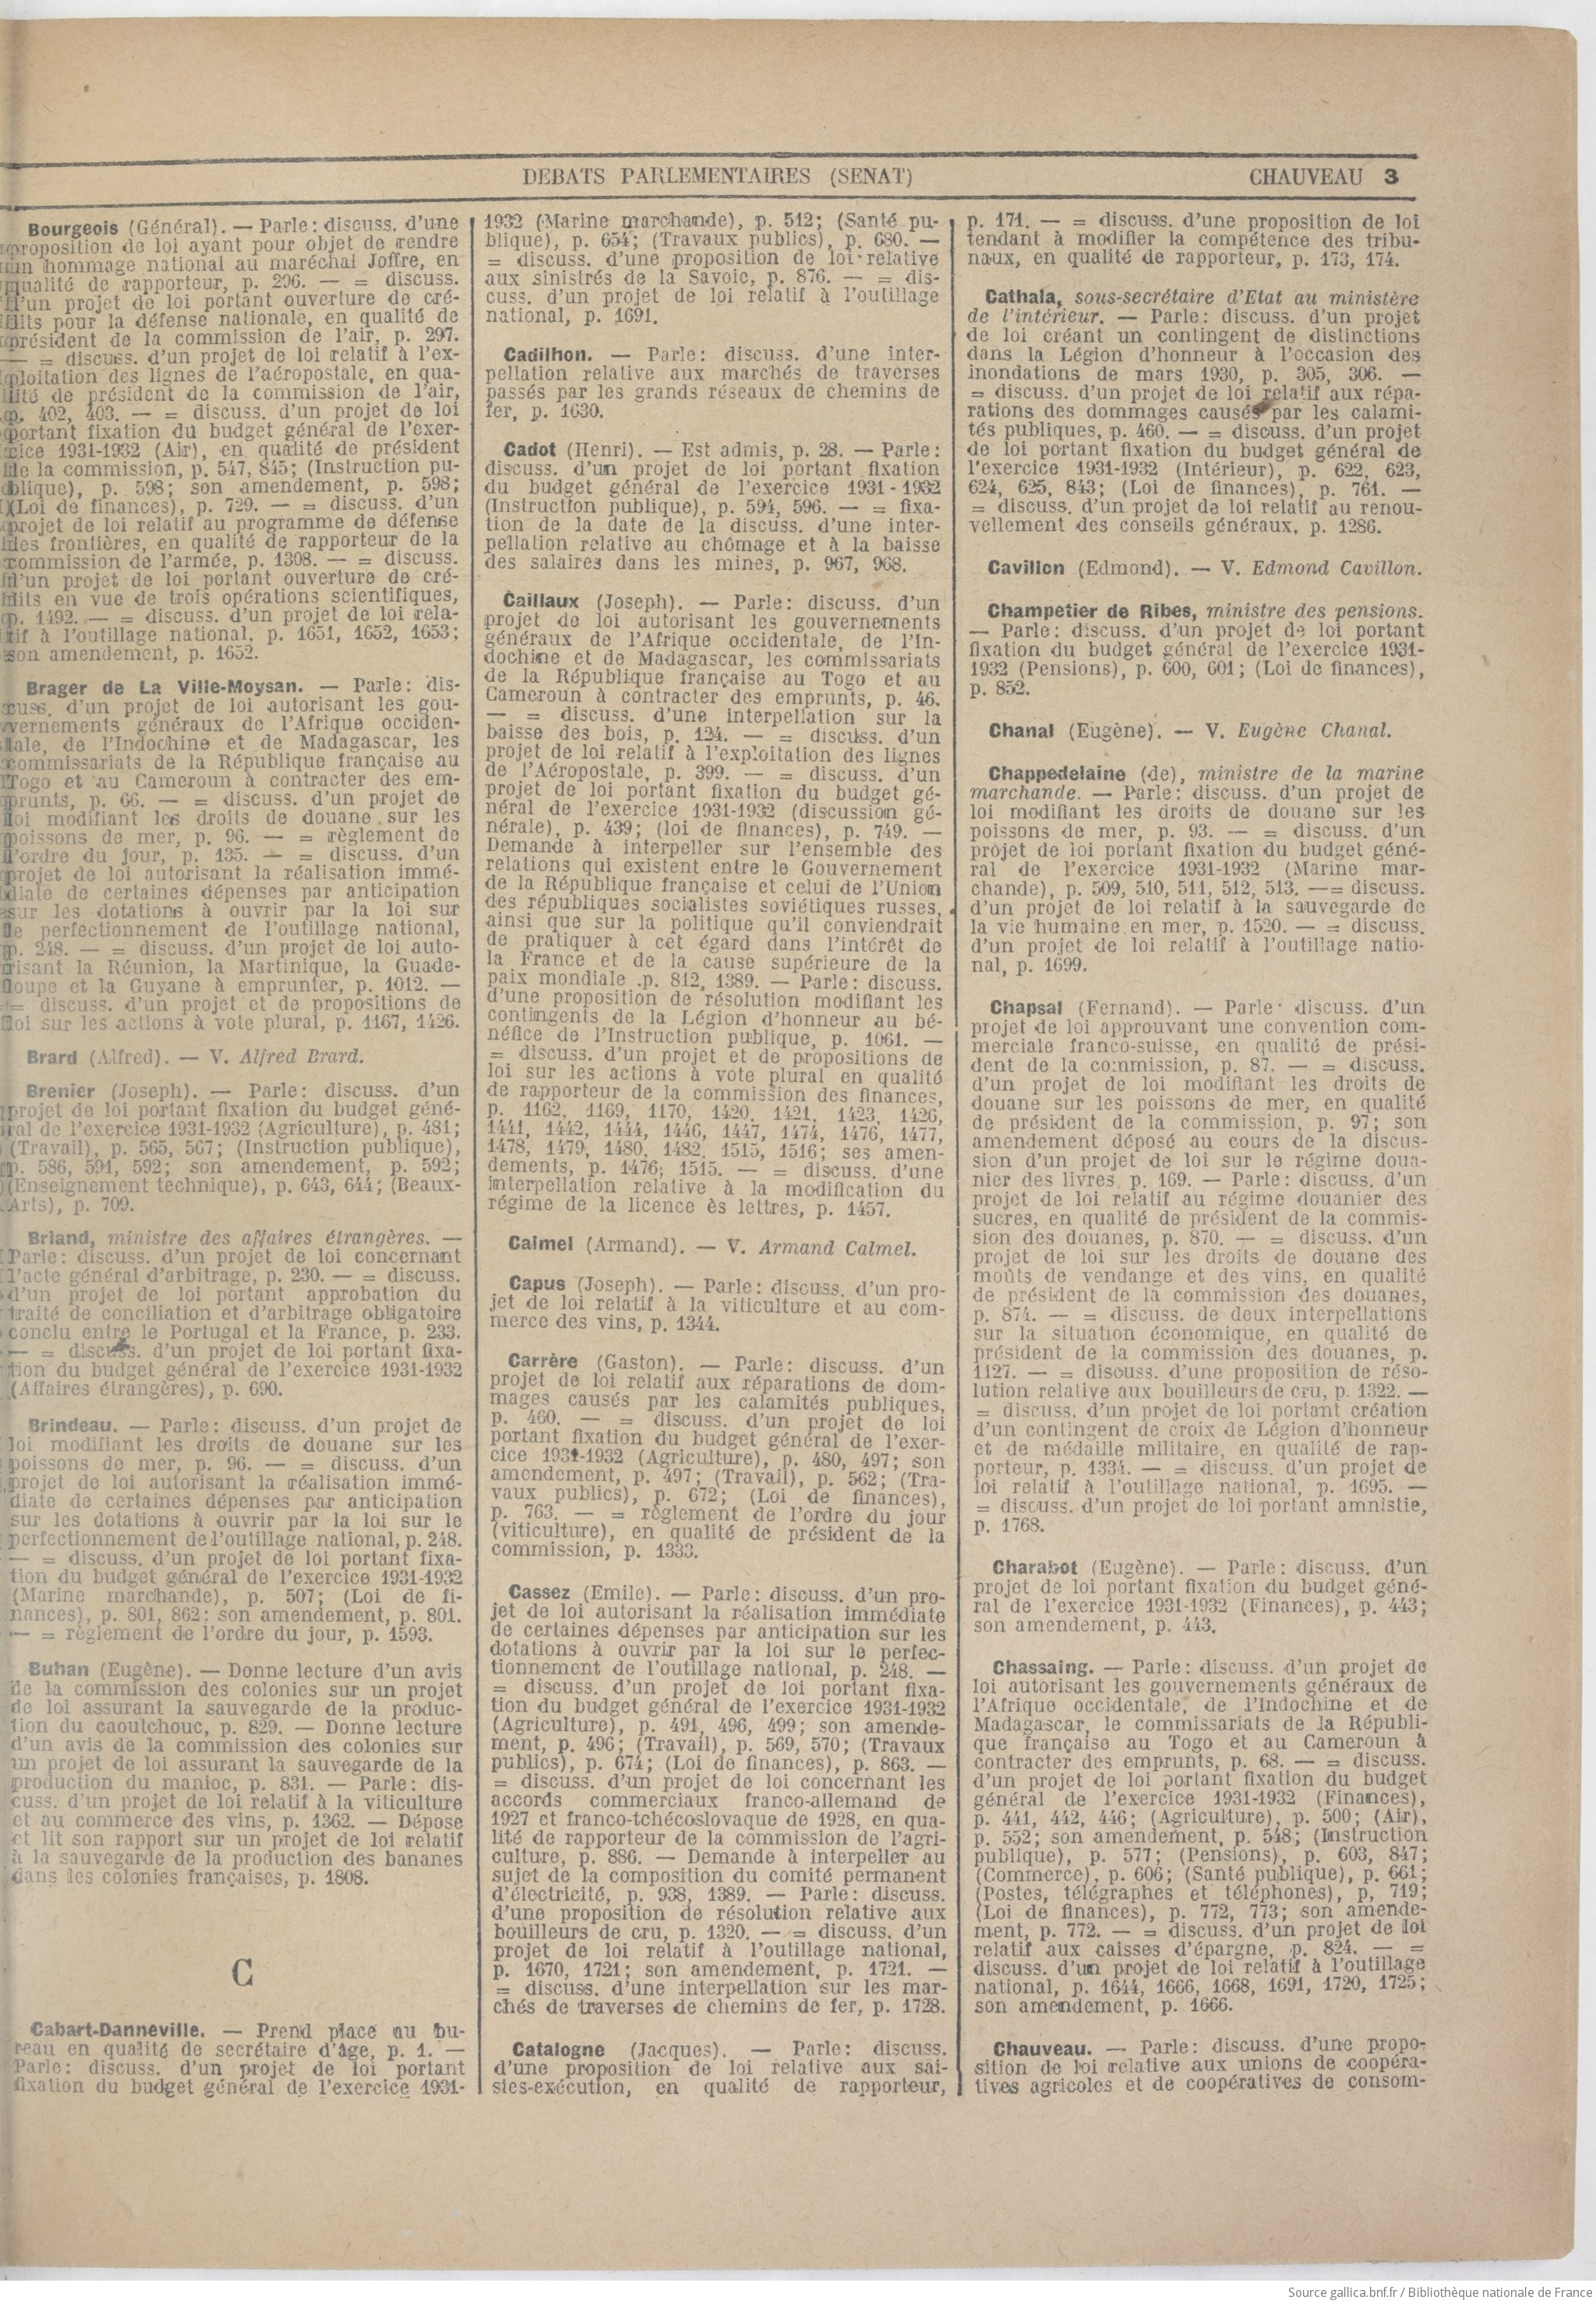
\includegraphics[width=0.8\textwidth]{img/jo_entire.jpeg}
    \caption{A page from the 1931 Senate \textit{Table des Noms}}
    \label{fig:jo}
\end{figure}

\clearpage
\section{Full prompt} \label{appdx:full-prompt}
This appendix features an English translation of the complete prompt used in our experiment, visible in \Cref{fig:full_prompt}.
\begin{figure}[!h]
\begin{minipage}{\textwidth}
\small
\begin{verbatim}
<TASK TO DO>: Extract from the text I am about to give you,
information from each entry, each of which relates to one person.
<NEED TO KNOW>: First of all, be aware that there is one entry per
person and that, for context, the people mentioned have participated
in the activity of the Senate. They are generally senators, ministers,
undersecretaries, etc.
<ENTRIES>: Each entry consists of: the NAME and sometimes the FIRST
NAME of a speaker (str); sometimes his role (this is not always
specified); a list of ACTIONS he has performed or which concern him.
<ACTION>: Each action concerning a speaker is generally linked to one
or more page numbers. When there is a page reference, you can be sure
that it is a reference to an action concerning the stakeholder.
<INDEX REFERENCE CASE>: In the case where an entry does NOT set out
actions or facts and/or pages concerning a speaker, but a simple
nominal mention, then it is an index reference. In this case, you
should indicate the reference of the reference (str). These references
are generally the first names and surnames of contributors. These
references therefore do not refer to pages, but to other nominal
entries.
<HERE IS THE INFORMATION TO BE EXTRACTED>: So I want you to give me
the surnames (and first names if there are any); as well as the page
numbers relating to the descriptions of the actions or interventions
of each speaker -- List[int]-- OR, if there is no action, just say
that it is an index reference ("<index reference>") -- (str).
<NOTE>: - When there is no index reference (a str), adopt this syntax
at the appropriate level: "references_pages":"<index_reference>".
- First names must be placed in brackets and after the name.
- If a page reference appears several times in an entry (i.e. for the
same speaker), there is no need to repeat it.
<ATTENTION>: The text submitted to you may be truncated. If this is
the case, ignore the incomplete text and consider only the complete
entries.
SO HERE IS THE TEXT from which you need to extract the information:
\end{verbatim}
\end{minipage}
\caption{Submitting a request to an LLM via a the Mistral API, including entity extraction instructions, the raw text, and the expected data schema. }
\label{fig:full_prompt}
\end{figure}

\clearpage
\section{Full data schema}
\label{appdx:schema}
\begin{figure}[H]
\small
\begin{verbatim}
class Speaker(BaseModel):
    name: str = Field(..., description="Name (and first name if applicable)")
    page_references: List[int] = Field(..., 
        description="List of page numbers where the speaker is referenced, 
        else <index cross-reference>")

class SenatorsInterventions(BaseModel):
    list_of_speakers: List[Speaker] = Field(..., 
        description="List of all speakers")
\end{verbatim}
\caption{Simplified data schema defined using Pydantic. Each participant is described by a name and a list of page numbers, which serve as indirect temporal markers. Description fields embedded in the schema act as semantic tags, guiding the language model in entity extraction.}
\label{fig:pydantic_schema}
\end{figure}

\clearpage
\section{Full experimental results}\label{appdx:full-results}
%TODO add all 3 tables here, properly identifying the ones in the main paper and the others

\begin{table}[htbp]
\centering
\begin{adjustbox}{width=\textwidth, center}
\begin{tabular}{lrrrrrr}
\toprule
Source & Precision (Biased) & Recall (Biased) & IMQ & Ground Truth Entries & Predicted Entries & Matches \\
\midrule
page 02 & 1.0000 & 1.0000 & 0.9513 & 23 & 23 & 23 \\
page 03 & 1.0000 & 1.0000 & 0.9430 & 25 & 25 & 25 \\
page 04 & 1.0000 & 1.0000 & 0.9821 & 19 & 19 & 19 \\
page 05 & 1.0000 & 1.0000 & 0.8778 & 19 & 19 & 19 \\
page 10 & 1.0000 & 1.0000 & 0.8966 & 23 & 23 & 23 \\
\bottomrule
\end{tabular}

\end{adjustbox}
\caption{Results for deemed-perfect OCR}
\label{tab:summary}
\end{table}


\begin{table}[htbp]
\centering
\begin{adjustbox}{width=\textwidth, center}
\begin{tabular}{lrrrrrr}
\toprule
Source & Precision (Biased) & Recall (Biased) & IMQ & Ground Truth Entries & Predicted Entries & Matches \\
\midrule
page 02 & 1.0000 & 1.0000 & 0.9513 & 23 & 23 & 23 \\
page 03 & 1.0000 & 1.0000 & 0.9430 & 25 & 25 & 25 \\
page 04 & 1.0000 & 1.0000 & 0.9821 & 19 & 19 & 19 \\
page 05 & 1.0000 & 1.0000 & 0.8778 & 19 & 19 & 19 \\
page 10 & 1.0000 & 1.0000 & 0.8966 & 23 & 23 & 23 \\
\bottomrule
\end{tabular}

\end{adjustbox}
\caption{Results for OCR based on manual segmentation}
\label{tab:summary}
\end{table}

\begin{table}[htbp]
\centering
\begin{adjustbox}{width=\textwidth, center}
\begin{tabular}{lrrrrrr}
\toprule
Source & Precision (Biased) & Recall (Biased) & IMQ & Ground Truth Entries & Predicted Entries & Matches \\
\midrule
page 02 & 1.0000 & 1.0000 & 0.9513 & 23 & 23 & 23 \\
page 03 & 1.0000 & 1.0000 & 0.9430 & 25 & 25 & 25 \\
page 04 & 1.0000 & 1.0000 & 0.9821 & 19 & 19 & 19 \\
page 05 & 1.0000 & 1.0000 & 0.8778 & 19 & 19 & 19 \\
page 10 & 1.0000 & 1.0000 & 0.8966 & 23 & 23 & 23 \\
\bottomrule
\end{tabular}

\end{adjustbox}
\caption{Results for raw OCR, without segmentation or correction}
\label{tab:summary}
\end{table}


\begin{comment}
\section{Full data schema}
TODO indiquer modèle avec la gestion des renvois
\joel{Le modèle est déjà complet dans l'article }
\end{comment}


\end{document}
